\section{System Model}
\label{sec:system_model}

\begin{figure}[!htbp]
  \centering
  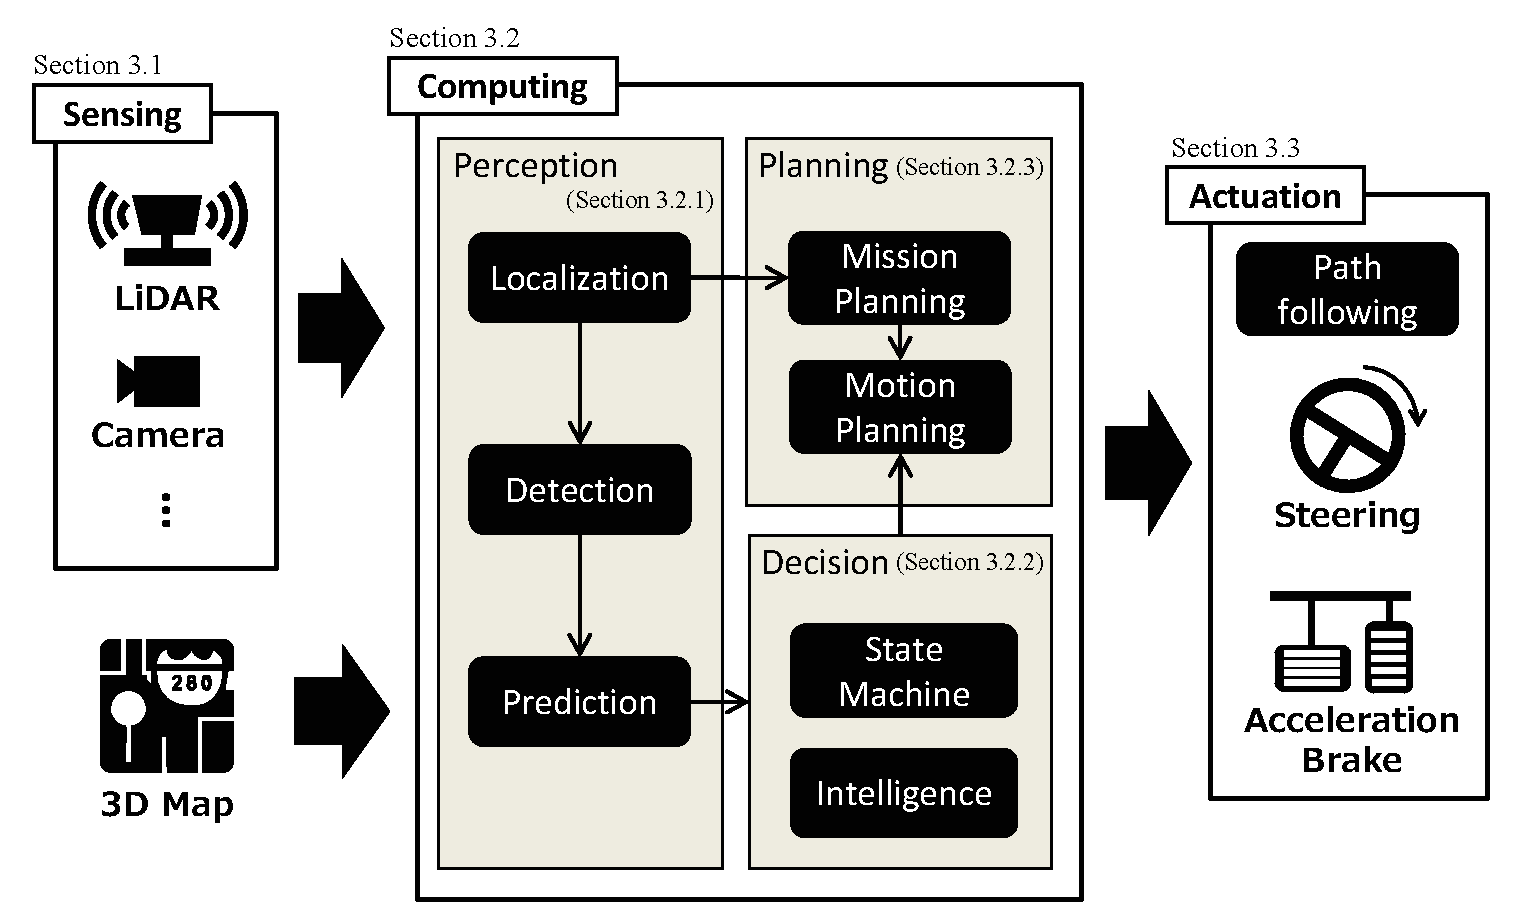
\includegraphics[width=0.6\linewidth]{../figure/system_model.eps}
  \caption{\label{fig:system_model}
    Basic control and data flow of autonomous vehicles.}
\end{figure}

Autonomous vehicles as cyber-physycal systems can be abstracted by
sensing, computing, and actuation, as shown in Figure
\ref{fig:system_model}.
Preferred sensing devices for urban-area self-driving, in particular,
include laser scanners (LiDAR) and cameras.
Actuation corresponds to manipulation of steering and stroking whose
twisted control commands are often generated by the path following module.
The computing intelligence is the major part of self-driving technology.
For instance, scene recognition requires localization, detection, and
prediction modules, while path planning falls into mission-based and
motion-based modules.
Each module employs corresponding algorithms.
Those implemented in Autoware, in particular, are introduced in Section
\ref{sec:autoware}.

Figure \ref{fig:system_model} shows a basic control and data flow of
autonomous vehicles.
Sensing devices acquire environmental information as input data for the
computing intelligence.
3D maps are also becoming more and more commonplace for self-driving
technology, especially for urban areas, to complement sensing and
computing capabilities of autonomous vehicles by high-definition and
high-resolution geographical information.
Leveraging these pieces of information, for example, the accuracy of
localization and detection can be improved highly without causing their
algorithms to become more complex.
Typical outputs of the computing intelligence are angular and linear
velocity values, which correspond to the commands for steering and
stroking, respectively.

\section{System Stack}

\begin{figure*}[!htbp]
  \centering
  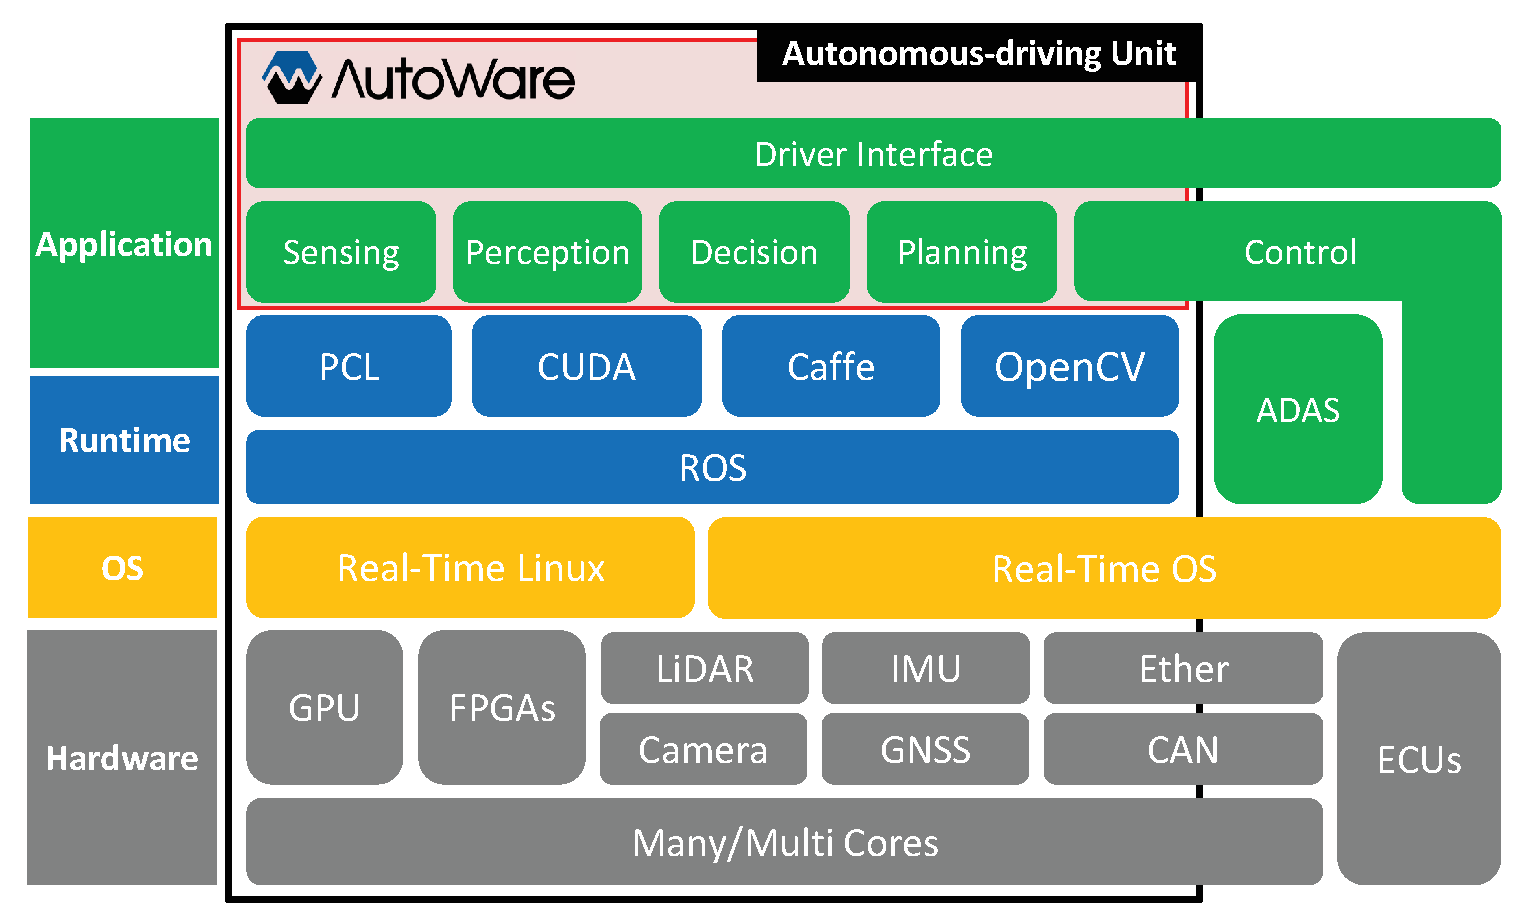
\includegraphics[width=0.6\linewidth]{../figure/system_stack.eps}
  \caption{\label{fig:system_stack}
  Complete system stack of autonomous vehicles using Autoware.}
\end{figure*}

We build the complete system stack of autonomous vehicles on top of
integrated platforms using open-source software, as shown in
Figure~\ref{fig:system_stack}.
The primary target of self-driving technology presented in this paper is
 set for urban areas rather than freeways and highways.
We develop Autoware which is a popular
open-source software project developed for urban-area autonomous
vehicles.
Autoware is based on Robot Operating System (ROS) and other
well-established open-source software libraries, as shown in
Figure~\ref{fig:system_stack}.
We introduce a brief overview of ROS separately in Section~\ref{sec:ros}.
Point Cloud Library (PCL) \cite{pcl} is mainly used to manage LiDAR
scans and 3D maps.
It is also used for data filtering and visualization.
CUDA \cite{cuda} is a programming framework for general-purpose
computing on GPUs (GPGPU).
Due to compute-intensive tasks in autonomous vehicles, GPUs and CUDA are
promising solutions for self-driving technology, though this paper does
not focus on them.
Caffe \cite{jia2014caffe}, \cite{caffe} is a native deep learning
framework made with expression, speed, and modularity in mind.
OpenCV \cite{opencv} is a popular computer vision library for image
processing.

Autoware provides a rich set of software packages, including sensing,
perception, decision making, planning, and control modules.
Many drive-by-wire vehicles can be transformed into autonomous vehicles
by installing Autoware.
In several countries, Autoware has already succeeded in demonstration of
autonomous vehicles driving for a long distance of public roads in urban
areas. 
Recently, automotive manufacturers and suppliers have also started
adopting Autoware as a baseline of their prototype autonomous vehicles.

In this section, we also briefly introduce hardware pieces of autonomous
vehicles assumed in this paper.
To apply our system stack, we need to make a modification to commercial
vehicles so that they can be controlled by external computers through
some secure gateway, and also install sensors on the vehicles.
The interface among the vehicles, computers, and sensors could be the
CAN bus, Ethernet, and/or USB 3.0.
The specification of sensors and computers, however, highly depends on
the functional requirement of each autonomous vehicle.
Autoware supports various sensing devices, but our prototype system
specifically uses Velodyne HDL-32e LiDAR scanners and PointGrey
Grasshopper3 cameras.
Autoware also supports various computers.
Many users often run Autoware on desktop and laptop computers.
In this paper, we specifically use NVIDIA DRIVE PX2, though our previous
work partly ported Autoware to another embedded computing platform,
called Kalray Massively Parallel Processor Array
(MPPA)~\cite{yuya2017exploring}. 

\section{Algorithms}
\label{sec:system_model}

In this section, we present the detail of Autoware in accordance with
Figure~\ref{fig:system_model}, with a particular emphasis on the modules
that we develop and extend for DRIVE PX2.
The remaining pieces of Autoware can be found and studied through its
project repositry~\cite{autoware}.
Note that Autoware is designed for urban-area autonomous vehicles, so we
may need alternative projects for those intended to drive on freeways
and highways.
Discussions on the accuracy and optimization of each algorithm are not
within the scope of this section.

\subsection{Sensing}
\label{sec:sensing}
Our system recognizes road environments, using various sensors, such
LiDAR scanners, cameras, radars, and GPS/IMU.
We use LiDAR scanners and cameras as primary sensing capabilities.
LiDAR scanners measure the distance to a target by illuminating that
target with a pulsed laser light and measuring the reflected pulses with
the scan.
Point-cloud data measured by LiDAR can be used to make digital
3D-representations of the environments.
Cameras are often used to recognize traffic lights and object classes,
which are sometimes superior to LiDAR scanners in terms of feature
quantity of objects and sampling rates.

Raw point-cloud data may need to be filtered and preprocessed before
proceeding to the computing stage.
For instance, we apply the Normal Distributions Transform (NDT)
algorithm \cite{biber2003normal} to 3D point-cloud data processing. 
Replacing the original points with one point of those centroids with
cubic lattice grid called a voxel, we can downsample data as approximate
points in the grid \cite{magnusson2009three}. 
This filter is applied before performing localization, detection, and
mapping.

In addition, radars and GPS/IMU can be used to further complement
localization, detection, and mapping.
Radars are already deployed in commercial vehicles, which are often used
for the purpose of ADAS safety applications.
GPS/IMU can be also coupled with gyro sensors and odometers to fix the
positioning information.

\subsection{Computing}
\label{sec:computing}

The computing intelligence is a major component of self-driving
technology.
Receiving sensor data and 3D maps as inputs, it computes the final path
trajectory as outputs to actuation components.
In this section, we explain its detail from the viewpoint of perception,
decision, and planning. 

\subsubsection{Perception}
\label{sec:perception}
The purpose of perception is to estimate of the position of the
ego-vehicle in the 3D map, and also to recognize surrounding scenes
including moving objects and traffic signals.

\textbf{Localization}:
Localization is one of the most basic and important tasks of autonomous
vehicles.
Especially in urban areas, the accuracy of localization dominates the
reliability of autonomous vehicles.
In Autoware, localization is based on scan matching with 3D maps and
LiDAR scanners, which achieves a few centimeters order of accuracy for
position and rotation. 
We use the NDT \cite{biber2003normal} algorithm to solve the
localization problem.
The computational cost of the NDT algorithm does not suffer from the map
size (the number of points).
Thus, we can use high-definition and high-resolution 3D map data in
real-time.
To be precise, we use the 3D version of NDT to perform scan matching
over filtered 3D point-cloud data and 3D map data by using PCL, as shown
in Figure \ref{fig:rviz_autoware} (b) \cite{magnusson2009three}.
As a result, localization meets an order of centimeters accuracy.

Localization is also a key technique for 3D mapping.
If autonomous vehicles are localized precisely in real-time, 3D maps can
also be continuously generated and updated by registering 3D point-cloud
data acquired at every 3D LiDAR scan.
This approach is often referred to as simultaneous localization and
mapping (SLAM).

We primarily use the NDT algorithm for both localization and mapping,
though Autoware also supports another well-known algorithm called
Iterative Closest Point (ICP).
This is a feature of Autoware that users can choose preferred algorithms
for their system.

% \begin{figure}[htbp]
%     \centering
%     \includegraphics[width=1.0\linewidth]{../figure/rviz_localization.eps}
%     \caption{\label{fig:rviz_localization}
%     NDT scan matching localization using a 3D map and a 3D LiDAR scan.}
% \end{figure}
  
\textbf{Detection}:
Once localized, we next have to detect surrounding objects, such as
vehicles, pedestrians, and traffic signals, to avoid accidents and
violation of traffic rules.
We first focus on moving objects (vehicles and pedestrians), while
Autoware is also capable of recognizing traffic signals and lights as
explained later in this section. 
Autoware supports deep learning \cite{liu2016ssd},
\cite{DBLP:journals/corr/RedmonF16} and pattern recognition
\cite{felzenszwalb2010object} for detection of vehicles and pedestrians,
using libraries such as Caffe and OpenCV. 
In particular, as shown in Figure \ref{fig:rviz_autoware} (c), we primarily use the Single Shot MultiBox Detector (SSD)
algorithm \cite{liu2016ssd} and the You only look once (Yolo2) algorithm
\cite{DBLP:journals/corr/RedmonF16}, which are based on deep learning.
They are unified frameworks for object detection with a single neural
network, realizing fast object detection in real-time.
On the other hand, the pattern recognition algorithm based on Deformable
Part Models (DPM) \cite{felzenszwalb2010object} searches and scores the
Histogram of Oriented Gradients features of target objects on the image
captured by a camera \cite{dalal2005histograms}.

Apart from image processing, we also use point-cloud data scanned from a
3D LiDAR scanner to detect objects by Euclidean clustering. 
Point cloud clustering aims to obtain the distance to objects rather
than to classify them.
The distance information can be used to range and track the objects
classified by image processing.

Assuming that localization is precise and a 3D map is built for the area
where the target autonomous vehicle is self-driving, we can improve the
accuracy of recognizing traffic signals and traffic lights.
Projecting the 3D map onto the image originated on the current position,
we know the exact road area on the image.
Therefore, we can constrain the region of interest (ROI) for image
processing to this road area so that we can save execution time and
reduce false positives.
To obtain ROI, we conduct calibration between the 3D LiDAR scanner and
the camera.
The calibration process needs to be done offline in advance.
We apply this approach to recognize traffic signals from the camera image as shown in Figures \ref{fig:rviz_autoware} (f) and (g).
In general, traffic light recognition is known to be one of the most
difficult problems for autonomous vehicles.
We can, however, achieve accurate traffic light recognition,
due to the presence of 3D map information and the result of precise
localization.

% \begin{figure}[htbp]
%     \centering
%     \includegraphics[width=1.0\linewidth]{../figure/rviz_detection.eps}
%     \caption{\label{fig:rviz_detection}
%     Object detection and traffic-light recognition with sensor fusion: (a) results of SSD objects detection, (b) projection of the 3D point-cloud data onto the image, (c) traffic-light positions of 3D map, (d) ROI and results of traffic-light recognition.}
% \end{figure}


\textbf{Prediction}:
Because we perform the object-detection algorithm on each frame of the image and point-cloud data, we must associate its results with other frames on a time basis so that we can predict the trajectories of moving objects for mission and motion planning.

We can use two algorithms, Kalman Filter and Particle Filter, to solve this prediction problem.
Kalman Filter is used under a linear assumption that our autonomous vehicle is driving at constant velocity while tracking moving objects \cite{kalman1960new}.
Its computational cost is lightweight and suited for real-time processing.
Particle Filter, on the other hand, can work for nonlinear tracking scenarios, in which both our autonomous vehicle and tracked vehicles are moving \cite{arulampalam2002tutorial}.
In our platform, we use both Kalman Filter and Particle Filter, depending on the given scenario.
We also apply them for tracking on both the 2D (image) plane and the 3D (point-cloud) plane.

We can combine detected and tracked objects on the image captured by the camera, and clustered and tracked objects obtained by the 3D LiDAR sensor.
This is often referred to as sensor fusion with projection and re-projection.
We conduct sensor fusion between 3D LiDAR sensors and cameras by beforehand calibration.

We augment scene recognition supported by our platform with sensor fusion of a camera and a 3D LiDAR sensor.
To calculate the extrinsic parameters required to make this sensor fusion, we must calibrate the camera and the 3D LiDAR sensor.
We can then project the 3D point-cloud information obtained by the 3D LiDAR sensor onto the image captured by the camera so that we can add depth information to the image and filter out the region of interest of object detection.
With sensor fusion, Figures \ref{fig:rviz_autoware} (d) and (e) represent the results of projection and bounding boxes of clustered 3D point-cloud objects projected onto the image.

The detected and tracked objects on the image can also be reprojected onto the 3D point-cloud coordinates using the same extrinsic parameters.
We also use the reprojected object positions to determine the motion plan and, in part, the mission plan.

\subsubsection{Decision}
\label{sec:decision}

After we recognize surrounding road environments such as obstacles and traffic signals, we can predict the trajectories of moving objects and make decisions for mission and motion planning.
This prediction and comprehensive decision components are under development in our autonomous-drive platform.

We adopt a state machine and machine learning intelligence for understanding, forecasting of a situation, and decisions according to the road scenarios.
Our platform enables the drivers to supervise state of the vehicle and makes comprehensive decisions for following planners.
Based on the results of this component, the suitable motion planner must generate trajectories depending on each scenario.

\subsubsection{Planning}
This component conducts trajectory planning on the basis of the comprehensive decision by above decision component.
We breakdown path planning into mission and motion planning.
We plan a global trajectory based on current location and destination, and then conduct basic local motion planning to determine the final path trajectory.
We can use graph-search algorithms such as hybrid-state A* search \cite{dolgov2010path}, and trajectory generation \cite{nagy2001trajectory} such as lattice-based algorithms \cite{darweesh2017open}.
% A demonstration video of the adaptation of OpenPlanner to Autoware can be seen at: https://www.youtube.com/watch?v=FKM8v79X3_s
We must choose the suitable planner with the decision component, depending on the road scenario.

\textbf{Mission planning}:
Under the traffic rules, our mission planner uses a rule-based mechanism to autonomously assign the path trajectory, such as for lane change, merge, and passing.
This mechanism is not completely autonomous in our platform.
The high-definition 3D map contains static road information for navigation and global planning.
In more complex scenarios, such as parking and recovering from operational mistakes, the driver can supervise the path.
In either case, once the path is assigned, the local motion planner is launched.

The basic policy of our mission planner is that we drive on the cruising lane throughout the route provided by a commodity navigation application based on the high-definition 3D map.
The lane is changed only when our autonomous vehicle is passing the preceding vehicle or approaching an intersection followed by a turn.

\textbf{Motion planning}:
The motion planner is a design knob for self-driving that corresponds to the driving behavior, which is not identical among users and environments.
Hence, our platform currently provides only a basic motion-planning strategy so that we are building a high-level intelligence for the comprehensive decision on top of this motion planning component.
Under the constraints of the current and goal state of the vehicle, the feasible trajectory must be dynamically  generated from the travelable area based on the 3D map information, considering the surrounding objects and traffic rules.

In unstructured environments, such as parking lots, we provide graph-search algorithms, such as A* \cite{hart1968formal} and hybrid-state A* \cite{dolgov2010path}, to find a minimum-cost path to the goal with a cost map, as shown in Figures \ref{fig:rviz_autoware} (h) and (i).
The graph-search algorithms can solve complex scenarios, although they sacrifice processing speed.
In structured environments, such as roads and traffic lanes, on the other hand, the density of vertices and edges is likely high and not uniform, which constrains the selection of feasible headings.
We, therefore, use conformal spatiotemporal lattice-based algorithms to adapt the motion plan to the environment \cite{mcnaughton2011motion}.
State-of-the-art research encourages the implementation of these algorithms \cite{urmson2008autonomous}.
Trajectories for obstacle avoidance and lane change must be calculated in real time with fast algorithms such as lattice-based algorithms \cite{pivtoraiko2009differentially}, \cite{mcnaughton2011motion}, and selected with an evaluation function, as shown in Figure \ref{fig:rviz_autoware} (j).

\subsection{Actuation}
\label{sec:actuation}
We control our autonomous vehicle to follow the path generated by the motion planner as mentioned above.

\textbf{Path following}:
We use the pure pursuit algorithm \cite{coulter1992implementation} to actuate our autonomous vehicle.
According to the pure pursuit algorithm, we break down the path into multiple waypoints, which are discrete representations of the path.
At every control cycle, we search for the close waypoint in the heading direction.
We limit the search to outside of the specified threshold distance so that we can relax the change in angle in the case of returning onto the path from a deviated position.
As shown in Figure \ref{fig:rviz_autoware} (k), the velocity and angle of the next motion are set to such values that bring the vehicle to the selected waypoint with predefined curvature.

We update the target waypoint accordingly until the goal is reached.
The vehicle keeps following updated waypoints and finally reaches the goal.
If the control of gas and brake stroking and steering is not aligned with the velocity and angle output of the pure pursuit algorithm because of some noise, the vehicle could temporarily get off the path generated by the motion planner.
Although we currently use simple PID controller to handle the vehicle, parameters highly depend on the vehicle and the controller is not sufficient to control the vehicle smoothly.
Localization errors could also cause the gap between the vehicle and outputs of the pure pursuit algorithm.
As a result, the vehicle could come across unexpected obstacles.
To cope with this scenario, our path follower ensures a minimum distance to obstacles, overwriting the given plan.
Our motion planner also updates the waypoints, considering obstacles on heading lane area.

\clearpage

\begin{figure*}[!htbp]
  \centering
  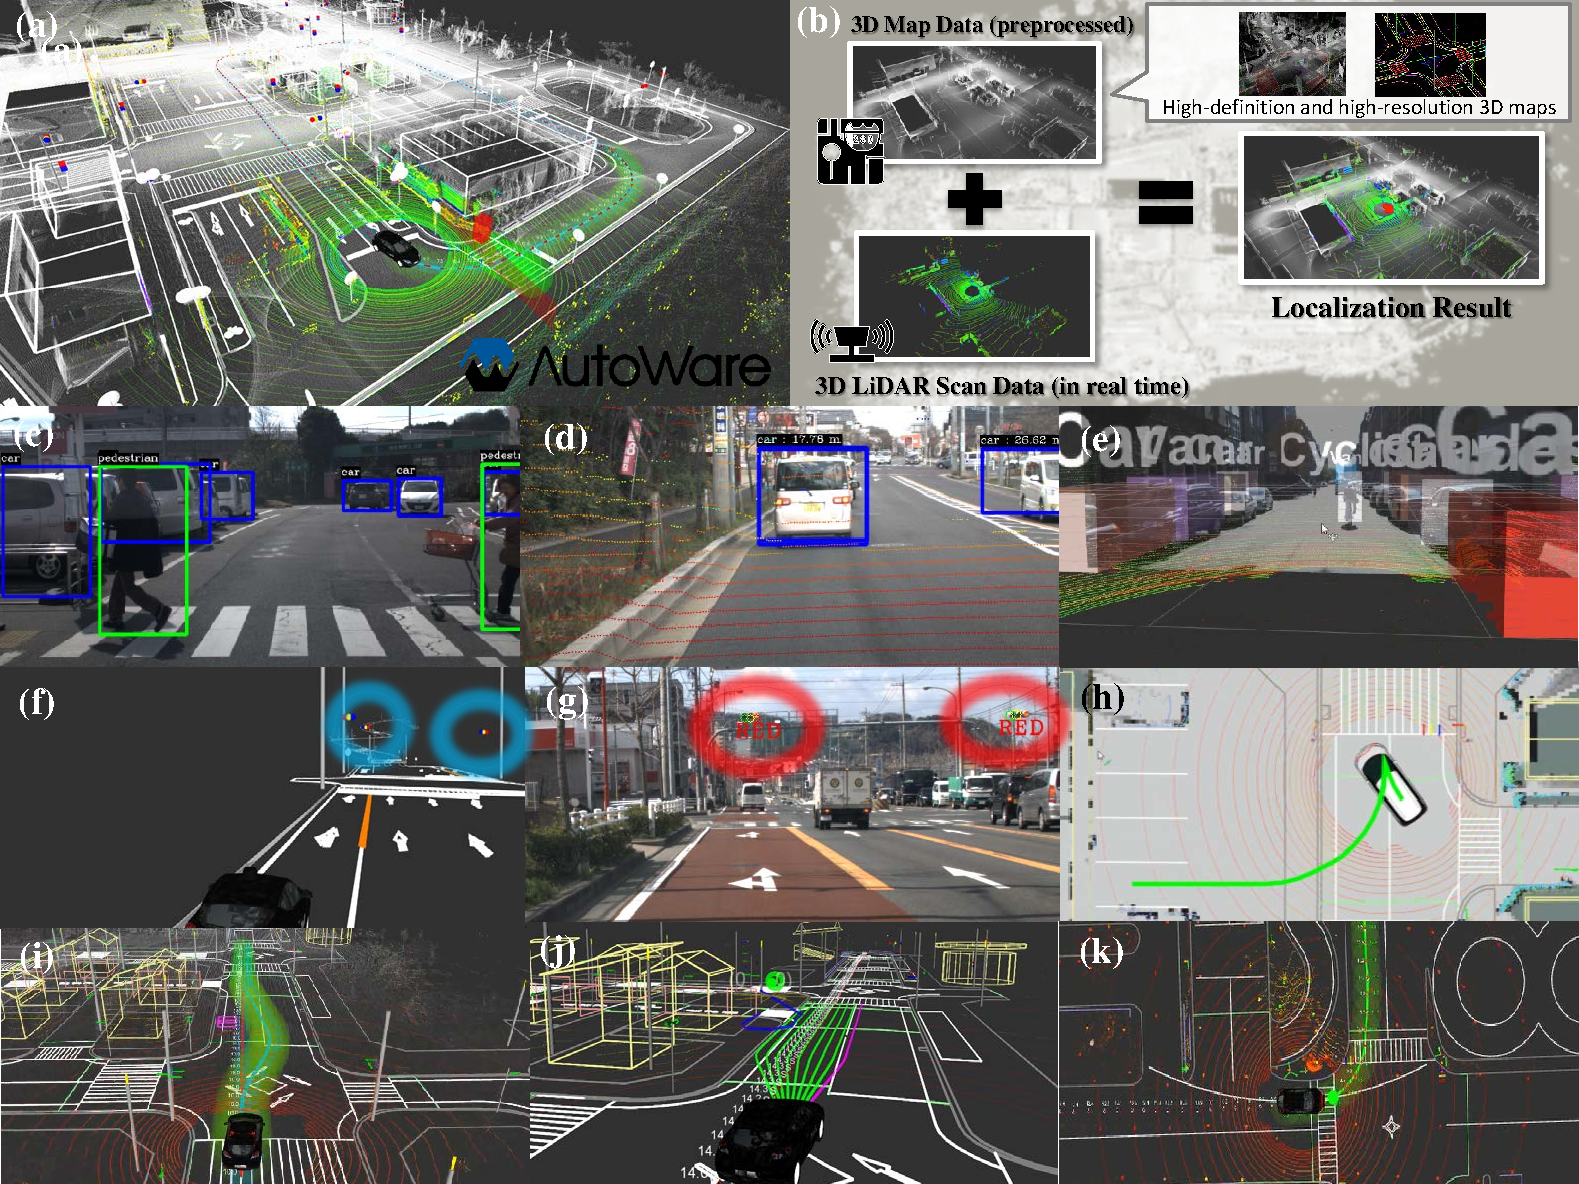
\includegraphics[width=1.0\linewidth]{../figure/rviz_autoware.eps}
  \caption{\label{fig:rviz_autoware}
  Self-driving software packages in Autoware:
  (a) RViz visualization with high-definition and high-resolution geographical information,
  (b) NDT scan matching localization using a 3D map and a 3D LiDAR scan,
  (c) deep learning based object detection with SSD, 
  (d) projection of the 3D point-cloud data onto the image, 
  (e) sensor fusion between the LiDAR sensor and the camera with calibration,
  (f) obtainment of the traffic light positions from the 3D map,
  (g) traffic light recognition with the ROI,
  (h) trajectory generation for parking lots using the hybrid-state A* search,
  (i) trajectory generation for object avoidance using the hybrid-state A* search,
  (j) trajectory generation for object avoidance using the lattice-based algorithm,
  (k) steering angular velocity calculation for path following using the pure pursuit algorithm.}
\end{figure*}
